\documentclass{article}
\usepackage{amsmath}
\usepackage{tikz}
\begin{document}

\title{Electricity and Magnetism - Lecture 5 Notes}
\author{Joshua Clement}
\maketitle

\section*{Electric Field of a Charge Distribution}
\begin{itemize}
    \item \textbf{Charge Density} (\(\lambda\)): Charge per unit length for a linear distribution.
    \item \textbf{Electric Field of a Charged Rod}:
    \begin{itemize}
        \item To determine the electric field, break the rod into small elements (\(\Delta q\)).
        \item Use the \textbf{superposition principle}: The total electric field is the sum of the contributions from each small charge element.
    \end{itemize}
\end{itemize}

\section*{Steps to Solve Charge Distribution Problems}
\begin{enumerate}
    \item \textbf{Understand the Geometry}: Identify the shape and distribution of the charged object.
    \item \textbf{Choose \(dq\)}: Define an infinitesimal charge element (\(dq\)).
    \item \textbf{Evaluate \(dE\)}: Determine the electric field contribution from \(dq\).
    \item \textbf{Exploit Symmetry}: Use symmetry to simplify calculations.
    \item \textbf{Set Up the Integral}: Integrate over the entire length/volume of the charge distribution.
    \item \textbf{Solve the Integral}: Compute the electric field by solving the integral.
    \item \textbf{Check Limiting Cases}: Ensure results are consistent for simpler configurations.
\end{enumerate}

\section*{Electric Field of a Finite Charged Rod in the Bisecting Plane}

\begin{figure}[h!]
    \centering
    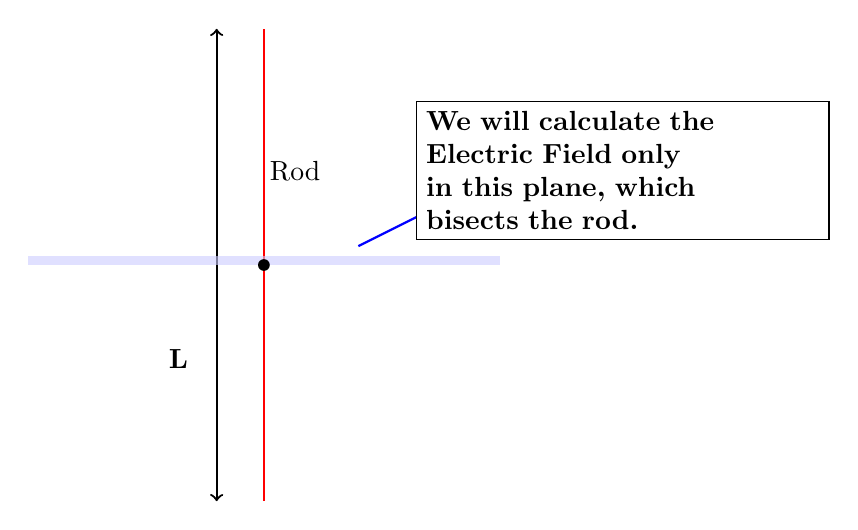
\begin{tikzpicture}[scale=1.2]
        % Draw the charged rod
        \draw[red, thick] (0, -2.5) -- (0, 2.5); % Rod from -L/2 to L/2
        \node[left] at (0.7, 1) {Rod};

        % Label the length of the rod
        \draw[<->, thick] (-0.5, -2.5) -- (-0.5, 2.5);
        \node[left] at (-0.7, -1) {\textbf{L}};

        % Draw the bisecting plane
        \fill[blue!20, opacity=0.6] (-2.5, 0) rectangle (2.5, 0.1);
        \node at (0, 0) [circle, fill=black, inner sep=1.5pt] {}; % Point at the intersection

        % Draw arrow and annotation box
        \draw[->, thick, blue] (1, 0.2) -- (2.2, 0.8);
        \node[draw, align=left, text width=5cm, fill=white] at (3.8, 1) {
            \textbf{We will calculate the}\\
            \textbf{Electric Field only}\\
            \textbf{in this plane, which}\\
            \textbf{bisects the rod.}
        };
    \end{tikzpicture}
    \caption{Illustration of calculating the electric field in the bisecting plane of a charged rod.}
    \label{fig:bisecting_plane}
\end{figure}

\begin{itemize}
    \item Consider a rod of length \(L\) with a uniform positive charge distribution.
    \item We calculate the electric field only in the plane that \textbf{bisects} the rod.
    \item \textbf{y-components cancel}, and only \textbf{x-components} contribute to the net electric field.
    \item Use the \textbf{superposition principle} to sum the contributions from each element (\(\Delta q\)).
    \item \textbf{Integral Representation}:
    \[
    \vec{E}_{\text{tot}} = \int_{-L/2}^{L/2} \frac{Qx}{4 \pi \epsilon_0 L (x^2 + y^2)^{3/2}} \, dy
    \]
    \item \textbf{None Integral Representation lol idk what its actually called}:
    \[
    \vec{E}_{\text{tot}} = (\frac{1}{4 \pi \epsilon_0}\frac{Q}{x\sqrt {x^2 +(\frac{L}{2})^2}})\hat{x}
    \]
\end{itemize}

\section*{Electric Field of an Infinite Rod}
\begin{itemize}
    \item For an \textbf{infinite rod}, the electric field is defined everywhere in space.
    \item \textbf{Linear Charge Density} (\(\lambda = \frac{Q}{L}\)): The electric field is dependent on the charge density.
    \item \textbf{Electric Field} at a distance \(r\) from the rod:
    \[
    E(r) = \frac{\lambda}{2 \pi \epsilon_0 r} \hat{r}
    \]
    \item The electric field decreases with distance (\(\frac{1}{r})\).
\end{itemize}

\section*{Key Takeaways: Charged Rods}
\begin{itemize}
    \item \textbf{Finite Rod}: The electric field is only calculated in the \textbf{bisecting plane}.
    \item \textbf{Infinite Rod}: The electric field extends \textbf{everywhere in space}.
    \item For a point far away from a finite rod (\(r \gg L\)), the electric field resembles that of a \textbf{point charge}.
\end{itemize}

\end{document}